
\chapter{Exceptional Control Flow}

\section{Exceptions}

이벤트 발생시에 예외 테이블이라고하는 점프 테이블을 통해서 운영체제에서 핸들러로 프로시저 콜을 하게한다.
그후에 제어를 다음 세가지중 하나로 처리한다.

\begin{enumerate}
    \item 현재 인스트럭션에 돌려준다
    \item 다음 인스트럭션으로 돌려준다 
    \item 프로그램을 종료한다.
\end{enumerate}

예외에는 하드웨어,소프트웨어 사이에서 각각 일어날 수 있으며 각각의 프로세서,OS 설계자가 예외를 미리 정해놓고 시스템 부팅시에 점프테이블에 할당하여 쓰는식.

예외 종류
\begin{itemize}
    \item inturrupt(비동기) : I/O에서 시그널  다음 인스트럭션으로 돌려준다.
    \item trap(동기) : instruction 실행결과. syscall로 OS단에서 처리,다음 인스트럭션으로 돌려준다.
    \item fault(동기) : ex) 가상 메모리 페이지 오류, 현재 인스트럭션으로 돌려준다.
    \item abort(동기) : 하드웨어 단의 복구불가능 에러, 프로그램 종료
\end{itemize}

syscall : 

리눅스에서 제공하는 syscall
\begin{itemize}
    \item read
    \item write
    \item open
    \item close
    \item stat
    \item mmap
    \item brk
    \item dup2
    \item pause
    \item alarm
    \item getpid
    \item fork
    \item execve
    \item \_exit
    \item sait4
    \item kill
\end{itemize}


\section{Processes}

프로세스 생성에는 두가지 종류가있다.

리눅스 프로세스 제어는 unistd.h에 함수가 정의되어 있다.
\begin{itemize}
    \item fork : 새로운 메모리에 매핑하여 자식프로세스로서 호출
    \item exevce : 현재 실행되는 프로그램의 메모리에 덮어쓰워 프로세스를 호출
\end{itemize}

exevce는 실행할 프로그램에 argv(인자리스트)와  envp(환경변수)를 보낼수있다

\begin{figure}[h!]
    \centering
    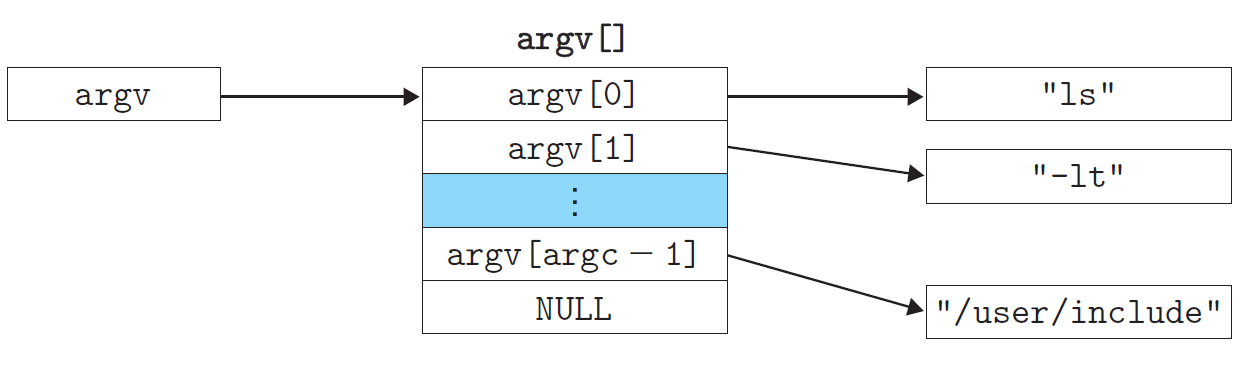
\includegraphics[scale=0.5]{pic/section8/pic1}
    \caption{Organization of an argument list.}
\end{figure}


\begin{figure}[h!]
    \centering
    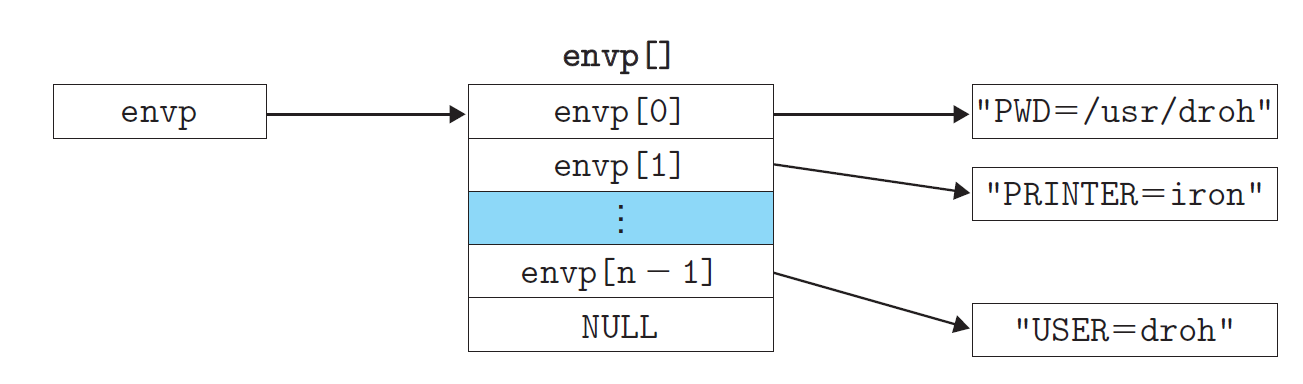
\includegraphics[scale=0.47]{pic/section8/pic2}
    \caption{Organization of an environment variable list.}
\end{figure}

\begin{figure}[h!]
    \centering
    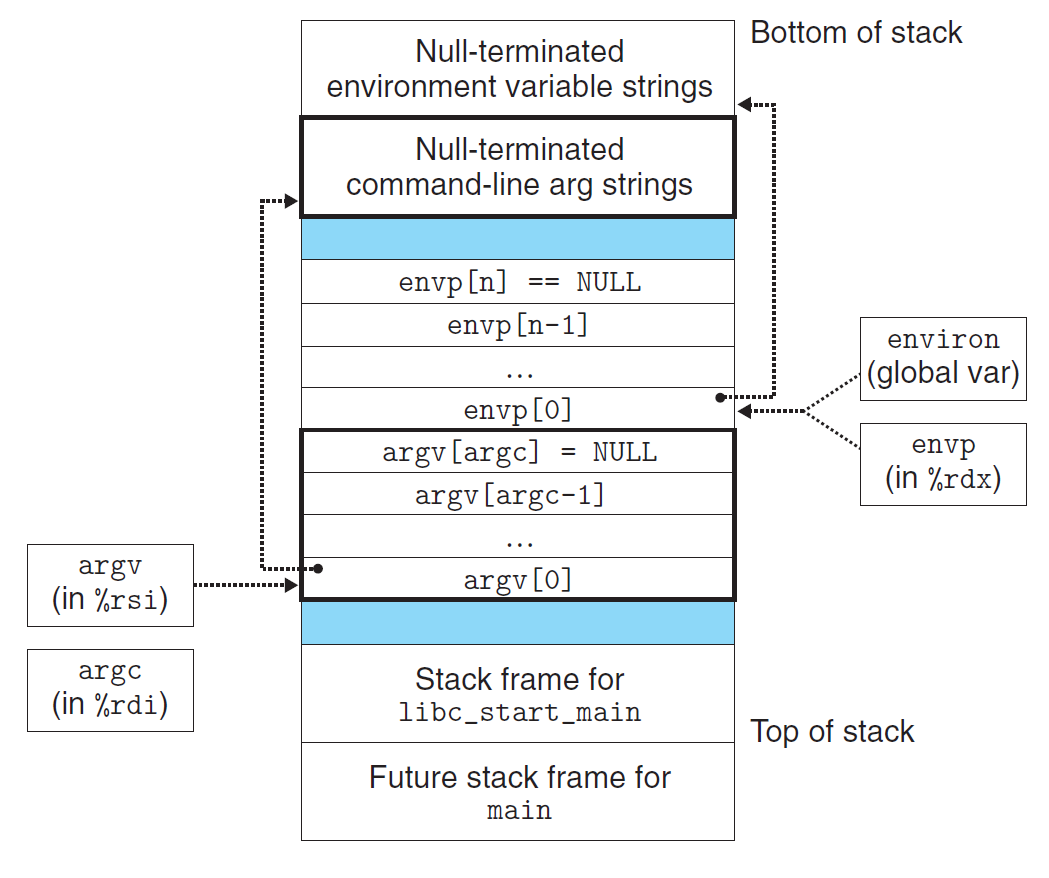
\includegraphics[scale=0.5]{pic/section8/pic3}
    \caption{Typical organization of the user stack when a    new program starts.}
\end{figure}



\section{Signals}


\section{Nonlocal Jumps}

setjmp longjmp

\section{Tools for Manipulating Processes}
